\documentclass{article}

\title {Online Order System}
\author{IDIR YACINE}
\usepackage{graphicx}

\usepackage{hyperref}
\hypersetup{
    colorlinks=true,
    linkcolor=blue,
    filecolor=magenta,      
    urlcolor=cyan,
    pdftitle={Overleaf Example},
    pdfpagemode=FullScreen,
    }


\begin{document}

\maketitle
\tableofcontents

\part{State of the art}
\section{general introduction}
\subsection{The Context}
The strengthening of interactions between trade and research institutions such as universities, colleges and research institutes has been increasingly seen as a strategic instrument for regional and national innovation, economic growth and competitiveness. The most recent innovation and research policies place a strong emphasis on interaction and cooperation between business and academia as a key public policy to foster innovation in the economy. Closer interaction is expected to lead to “more relevant research projects, faster uptake of scientific knowledge in the private sector, and better use of scientific knowledge” (NHD, 2003).
University-business interaction is highlighted as a tool to boost business research and development capacity building, as well as a tool to make higher education and research more relevant and responsive to business needs. This policy direction is part of the overall political vision of becoming a leading knowledge-based country in the global knowledge-based economy (NHD, 2003).
\subsection{The Project Objectives}
In our project we are too interested for creating a collaboration between informatique and Commerce fields, so actually we gave our interesting about "restaurant online orders” , restaurants are searching  for Target a larger segment of clients by using , ads , deliveration food , but now we suggest  a new way to solve their problem . 
Our platform is an intermediary that links customers and restaurants’. It helps the customer to reach his favorite restaurant easier. It also helps restaurants to expand their presence, especially in the information and Internet space, which will give the companies phone greater access to customers in terms of quality and quantity, and without Doubt will contribute to increasing sales and this is what companies of a commercial nature seek.
     Our platform is an exploitation of the scientific knowledge available in the field of informatics within the framework of digitizing trade and enhancing the presence of technology in daily transactions that would facilitate life and move from traditional methods to more modern methods commensurate with what the outside world has reached compared to our situation in Algeria .
\subsection{The MEMORY OVERVIEW}
\section{the project introduction }
\subsection{Introduction}
Our platform in particular, it's an orders management system, so in this chapter we will know what the “orders management system” is, and we will also discuss the goals that we are working to achieve through this work. We are interested in studying the existing criticisms, and suggest possible solutions.
Our mission is to create a system that consists of two parts, a client part, which is a mobile application in the Dart language and flutter framework and also Firebase, and there is a server part, which is only available to a store manager who manages orders, the server is a dynamique website that was created Using  CSS, HTML and ReactJS and Node Js frameworks , and managing databases using SQL, the role of this platform is to display products for sale via the mobile application, so that the order is managed through the store's manager through the website , the technology of order status tracking and automatic locator technology are available to facilitate the delivery of the ordered items, This platform also provides the ability to open a personal account   .
\subsection{Project objectives}
The objective of the project is to develop a platform that will allow
perform the following operations:
\begin{itemize}
\item make The ability to order food from the restaurant from anywhere     
\item organize food delivery operations.    
\item Manage clients orders.
\item show the restaurant products .
\end{itemize}
\subsubsection{the existence study}
So that restaurants can solve the problems they may face, including the problems of limited customers and lack of sales, they are forced to choose a suitable place where business is thriving and where people are interesting with food, or they are opening several branches in different places to expand business, which will cost them a lot of money and expenses. (Higher workplace expenses, equipment costs, higher wages for workers, higher taxes) It would run the risk of going bankrupt without making the required profit margin, and on the other hand the customer would have to go personally to the place of the restaurant to order food, which would waste time and effort and might find nothing to look for.  Now in our time, there are solutions to this crisis with minimal losses, especially with the presence of the Internet and informations technology, whose exploitation in our daily lives is necessary to facilitate many of the difficulties we faced in the past.
\subsubsection{the critique of the existence}
The current manual solution is traditional, thus posing different problems, namely: 
\begin{itemize}
\item It takes a long time to reach the desired goal .
\item It requires more effort with the risk of bankruptcy 
\item Requires a high budget and workers 
\item A solution that is not in line with the current development of trade methods with the spread of digitization and technology 
\item A traditional and imperfect solution to the problem at hand, as there are many factors that will directly affect this method 
\end{itemize}

\subsubsection{suggested solution}
Through information technology, new commerce and service fields development perspectives have emerged, and the creation of a restaurant order management application aims to develop and digitize e-commerce. Using the Internet as a means of dealing in the services and commercial sectors can reduce costs, improve performance and make dialy life citizens easier.
This project relies on the creation of a customer order management system.
\subsubsection{Client Section}
By creating a mobile application that is publicly available through which shops display their products and services and allow product demand in the presence of the Internet. It also determines the geographic location of the customer to assist in the delivery process. It also requires the opening of a personal account to create a client's profile to provide greater protection and ease to the customer.
\subsubsection{Administrator section}
The system also contains a section for store manager , which is a web site that allows for the control of the products offered, the reception and examination of customers' orders and the identification of the customer.
the system is Available in offline mode
\part{Project Methologies}
\section{Agile Developement}
\subsection{Continous Integration}
Continuous integration is a DevOps software development practice where developers regularly merge their code changes into a central repository, after which automated builds and tests are run. Continuous integration most often refers to the build or integration stage of the software release process and entails both an automation component (e.g. a CI or build service) and a cultural component (e.g. learning to integrate frequently). The key goals of continuous integration are to find and address bugs quicker, improve software quality, and reduce the time it takes to validate and release new software updates.
\subsection{GitHub}
Github is a Version control system that records changes to a file or set of files over time so that you can recall specific versions later.
It allows you to revert files back to a previous state, revert the entire project back to a previous state, compare changes over time, see who last modified something that might be
causing a problem, who introduced an issue and when, and more. Using a VCS also generally
means that if you screw things up or lose files, you can easily recover. In addition, you get all this for very little overhead.
\subsection{Code Quality}
\textbf{Single-Responsibility Principle} : A class should have one and only one reason to change, meaning that a class should have only one job.\\
\textbf{Open-Closed Principle} : Objects or entities should be open for extension but closed for modification.\\
\textbf{Liskov Substitution Principle} : Let q(x) be a property provable about objects of x of type T. Then q(y) should be provable for objects y of type S where S is a subtype of T.\\
\textbf{Interface segregation principle} :A client should never be forced to implement an interface that it doesn’t use, or clients shouldn’t be forced to depend on methods they do not use. \\
\textbf{Dependency Inversion Principle} : Entities must depend on abstractions, not on concretions. It states that the high-level module must not depend on the low-level module, but they should depend on abstractions.
\subsection{Test Driven Developement}
Test Driven Developement is an aproach that allow developers to deploy software features without the fear of breaking existing code which promote teams continous integration cycles.It also enhance softwares lifetimes and developement costs on the long run.

\textbf{How to write Tests}
Not all the code is created equally, only test the critical parts that contribute to the software sucess .
Write tests before production code to ensure software testibility and further enhanche code quality .
Name tests using their side effects,expected result or the state they leave the system in. 

\textbf{Why write Tests}
Softwares that has long lifetimes tend to grow exponentially in both complexity and developements costs as such TDD help us break down the complexity by providing live documentations in the form of tests .
They also work as a safety net to help future updates and maintenance .

\textbf{When not to write Tests}
Tests are not always the right answer as they slow down early developement and don't bring much to small,simple,short lived projects .

\section{Project Architecture}
\subsection{Analysis Models}
An analysis model is a byproduct of defining conceptual models that capture system behaviors,rules and information flows.Which help identifying the key requirements and obstacles of buidling the software.\\
\textbf{Key Points}
\begin{itemize}
\item Distiling the system into subsystems and capturing the relations between each.
\item Capturing the system core components ,events and ressources flows(REA).
\end{itemize}

\subsection{Domain Driven Design}
Domain Driven Design is an approach enabling teams to effectively manage construction and maintenance of complex domains software by seperating technical concerns from buisness logic and promoting agile enviroments.\\
\textbf{Key Points}
\begin{itemize}
\item Architecting the software into Ui,Application,Domain Infrastructure.Each layer would be further architected into bounded contexts.
\item Setting up knowledge-crunching sessions with domain experts whenever possible to develop a common ubiquitous language.
\item Identifying core and subdomains to better spend ressources on what really matters. 
\end{itemize}

\subsection{Design Patterns}
Design patterns are typical solutions to commonly occurring
problems in software design. They are like pre-made blue-
prints that you can customize to solve a recurring design prob-
lem in your code.
\textbf{Observer Pattern}\\
\textbf{Singeleton Pattern}\\
\section{Technologies}
\subsection{TypeScript}
A typed superset language that compile to javascript,it supports both commonJs and the latest release of EscmaScript formats.

\textbf{Why use it}
It reduces production errors by providing typing and autocomplete features.
Enables writing better and cleaner code as it introduces interfaces,classes,inheritance and access modifiers.

\textbf{DrawBacks}
Typescript is compiled to vanilla javascript before executing in the browser as such it requires a headder of pre-building it's modules.
Sometimes the compiled javascript is inefficent and ugly which might produce some performance bottlenocks.

\subsection{Sql}
Structured Query Language (SQL) is a programming language that is typically used in relational database or data stream management systems.
\subsection{Dart}
Dart is a client-optimized cross platform language , it adopts a declarative paradiagm which solves a lot of common problems in imperative languages . Dart is optimised for building ui as it provide hot reloading features . 
\section{TechStack}
\subsection{Flutter}
A cross-platform framework that enable developers to build visually enhanched apps,the framework use dart as it's underlying language and promotes a declarative programing paradigrams.
Projects built by flutter share most of their codebase throught the different platforms and provide communication channels to acess the platform specific  
features.

\textbf{Drawback : }
The framework is fairlly new and lack some crucial packages.
\subsection{NodeJs}
A javascript framework that enable building fast,responsive,scalable backend servers.However it's single threaded which makes it incompatable with intensive/cpu blocking operations.
\subsection{React}
A javascript framework that enables buidling single page applications,it also enhanches websites performances since it render on the client side instead of on the server.\linebreak
\textbf{Drawbacks:}
Since single page applications are rendered and cached on the client browser it produces some security overheads since it exposes all of the logic to the user.
The concern is easily dealt with by refactoring the backend logic into a different server and exposing said functionality through an api.
\subsection{Firebase}
Firebase is a platform and a framework developed by google that provide a range variety of services including authentication,hosting,cloud storage ,realtime database,firestore,functions,analytics and cloud computing.


\part{Project Implementation}
\section{Mobile client app}
\subsection{Project Structure}
\subsection{UI}
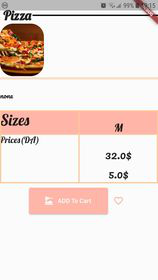
\includegraphics[scale=1]{./out/MobileApp/Ui/1.png}\\
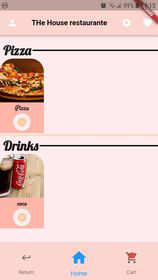
\includegraphics[scale=1]{./out/MobileApp/Ui/2.png}\\
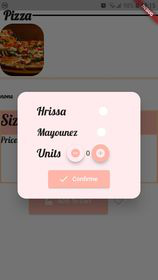
\includegraphics[scale=1]{./out/MobileApp/Ui/3.png}\\
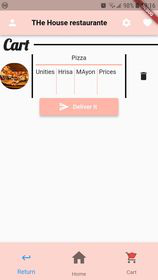
\includegraphics[scale=1]{./out/MobileApp/Ui/4.png}\\
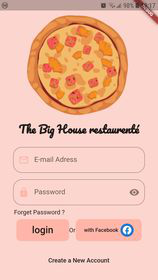
\includegraphics[scale=1]{./out/MobileApp/Ui/5.png}\\
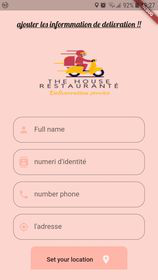
\includegraphics[scale=1]{./out/MobileApp/Ui/6.png}\\
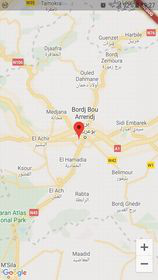
\includegraphics[scale=1]{./out/MobileApp/Ui/7.png}\\
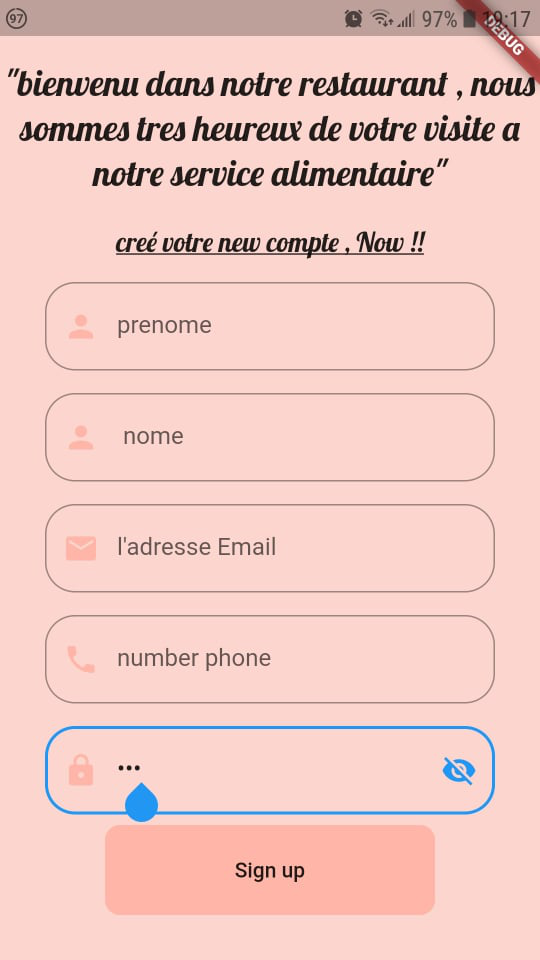
\includegraphics[scale=0.3]{./out/MobileApp/Ui/8.png}

\subsection{Application}
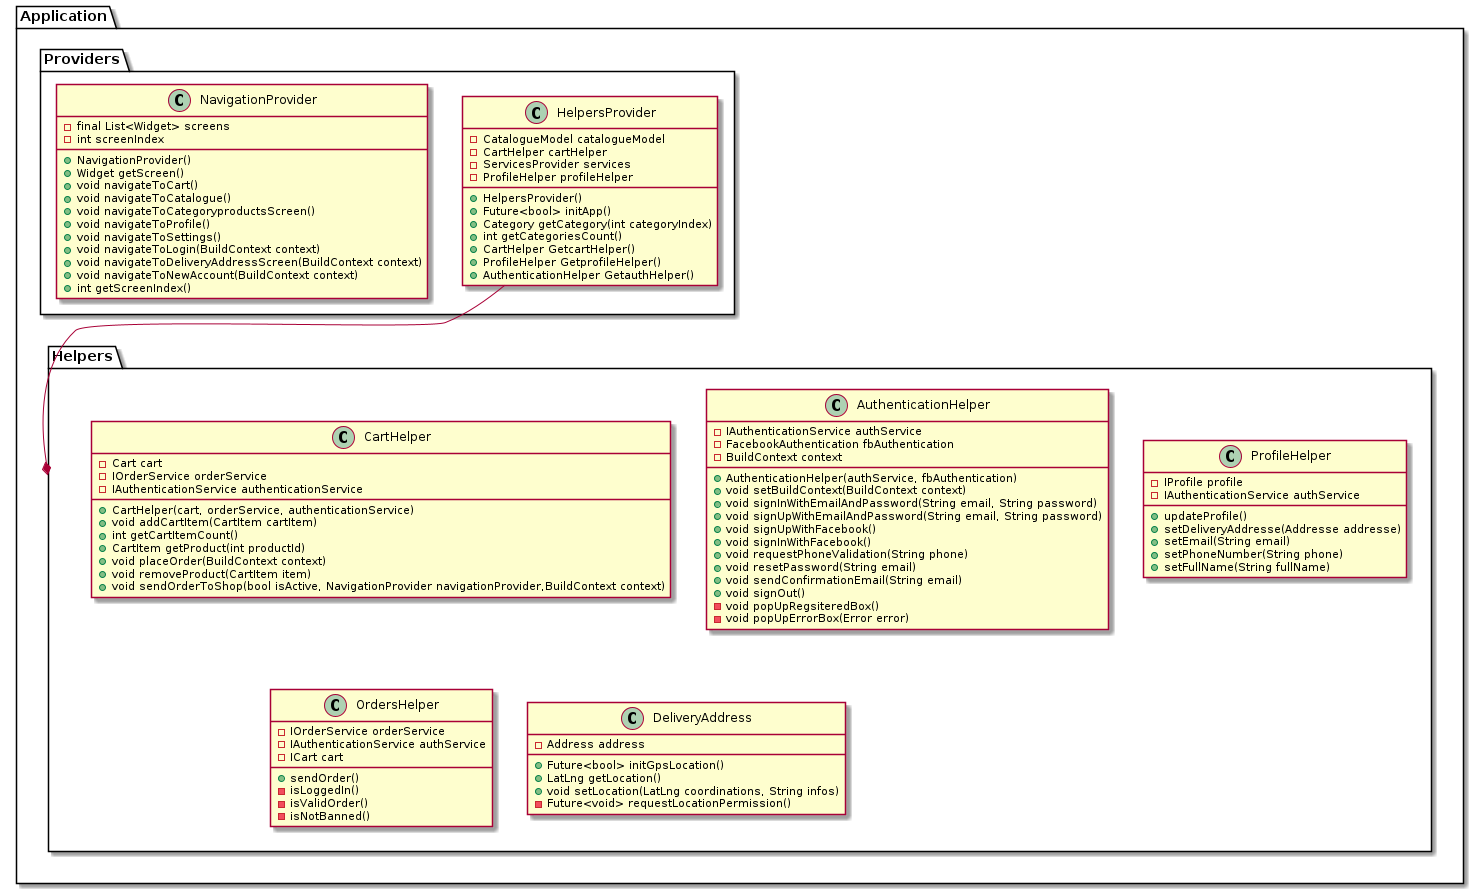
\includegraphics[scale=0.3]{./out/MobileApp/Application/Application.png}
\subsection{Domain}
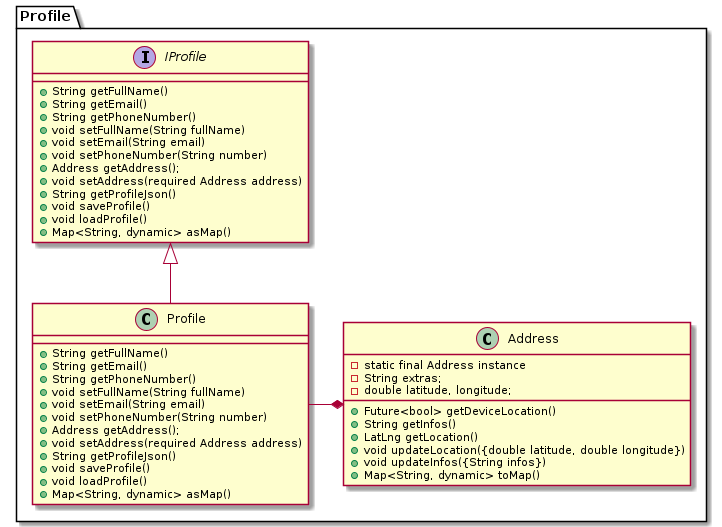
\includegraphics[scale=0.5]{./out/MobileApp/Domain/Profile/Profile.png}
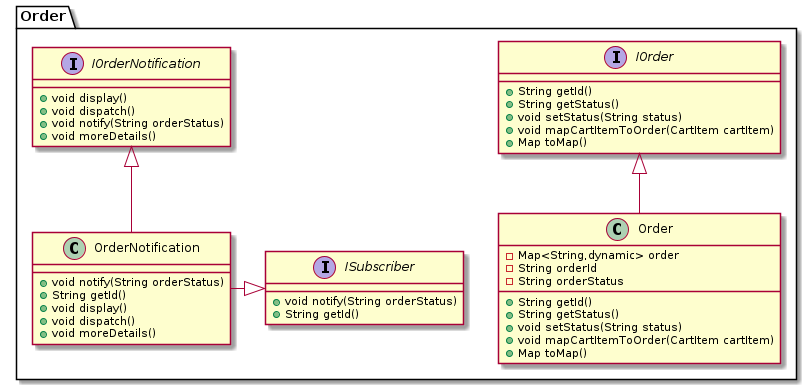
\includegraphics[scale=0.5]{./out/MobileApp/Domain/Order/Order.png}
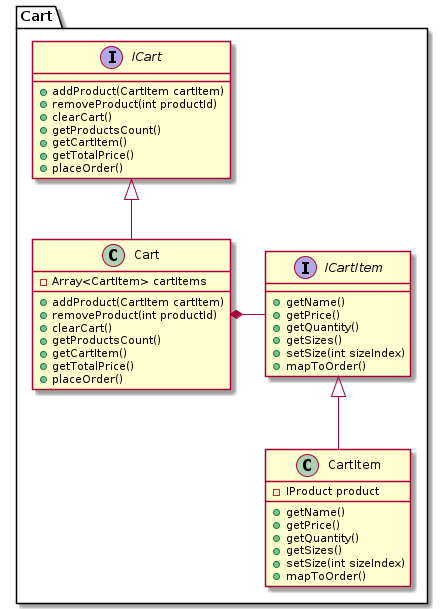
\includegraphics[scale=0.5]{./out/MobileApp/Domain/Cart/Cart.png}\\
\includegraphics[scale=0.5]{./out/MobileApp/Domain/Catalogue/Catalogue.png}

\subsection{Infrastructure}
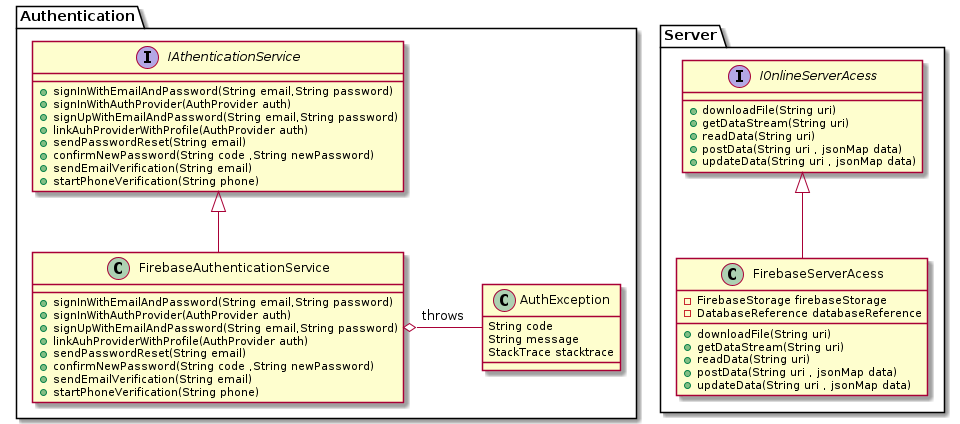
\includegraphics[scale=0.5]{./out/MobileApp/Infrastructure/infra.png}
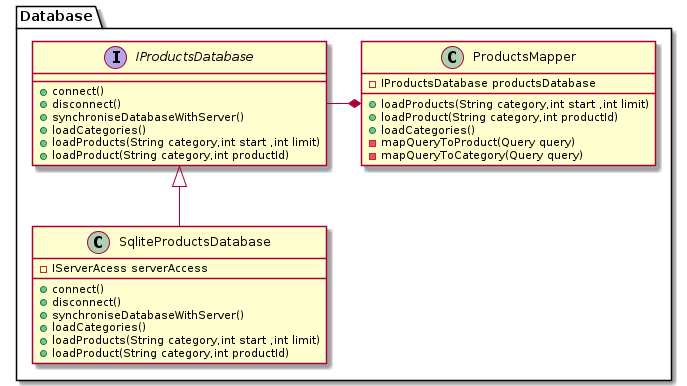
\includegraphics[scale=0.5]{./out/MobileApp/Infrastructure/infra3.png}\\
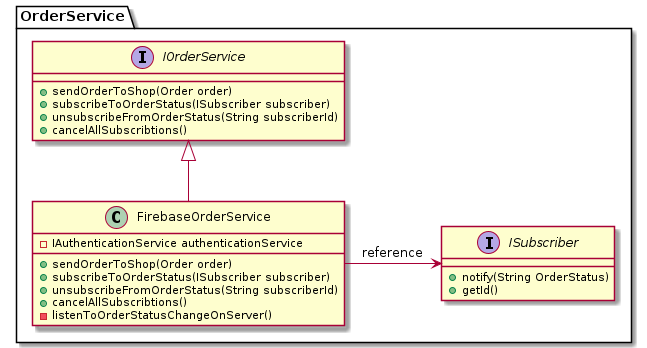
\includegraphics[scale=0.5]{./out/MobileApp/Infrastructure/infra2.png}
 
\section{Shop react app}
\subsection{Project Structure}
\subsection{UI}

\subsection{Application}
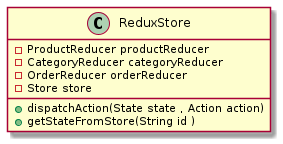
\includegraphics[scale=0.5]{./out/ReactApp/Application/ReduxStore/Store.png}\\
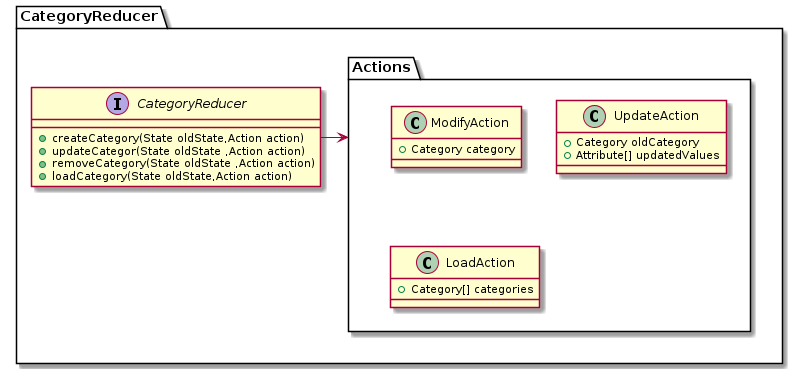
\includegraphics[scale=0.5]{./out/ReactApp/Application/ProductReducer/ProductReducer.png}\\
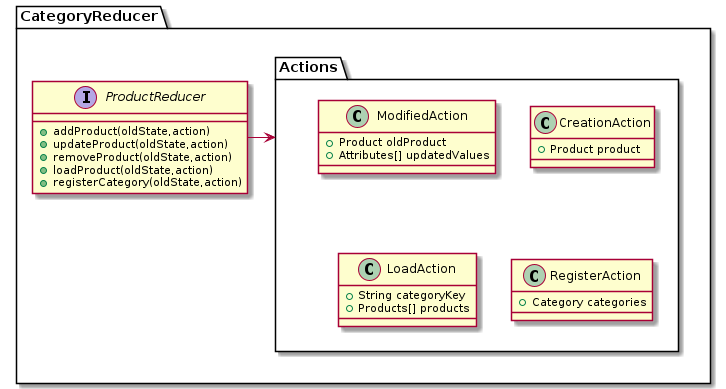
\includegraphics[scale=0.5]{./out/ReactApp/Application/CategoryReducer/CategoryReducer.png}\\
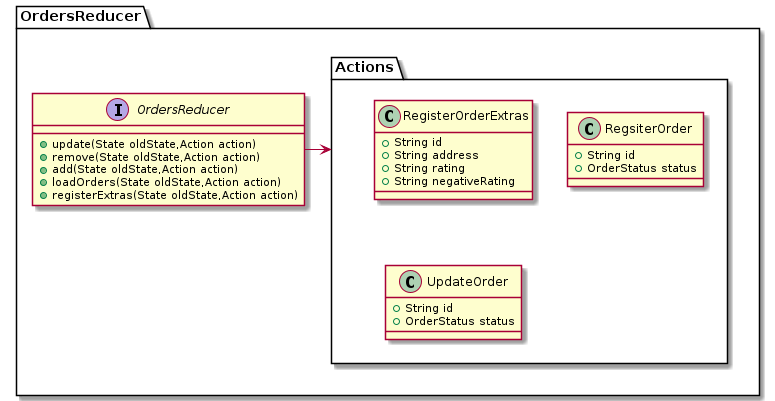
\includegraphics[scale=0.5]{./out/ReactApp/Application/OrdersReducer/OrdersReducer.png}\\

\subsection{Domain}
\subsection{Infrastructure}
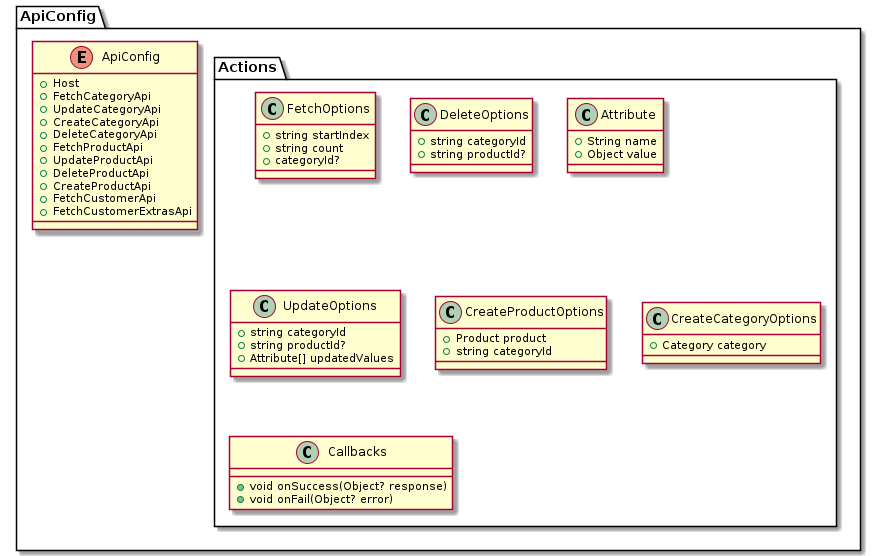
\includegraphics[scale=0.5]{./out/ReactApp/Infrastructure/ApiConfig/ApiConfig.png}\\
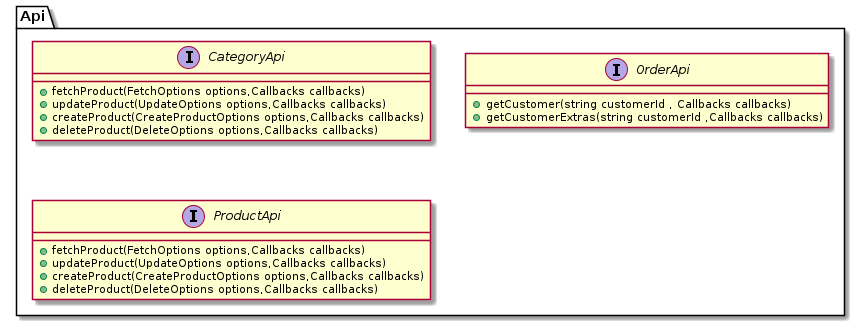
\includegraphics[scale=0.5]{./out/ReactApp/Infrastructure/Api/Api.png}
\section{Shop node app}
\subsection{Project Structure}
\subsection{Infrastructure}
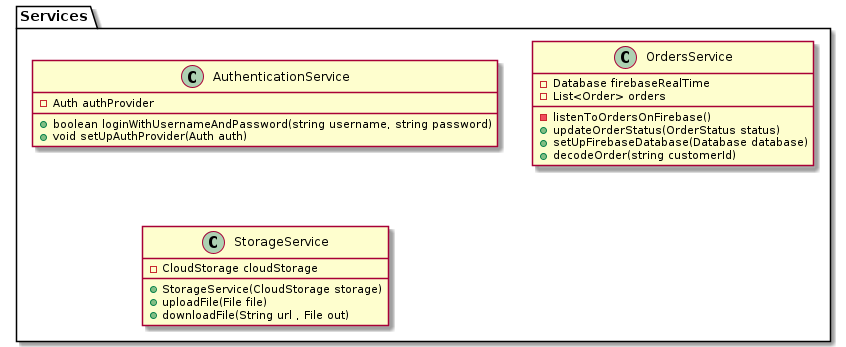
\includegraphics[scale=0.5]{./out/NodeApp/main/Services.png}
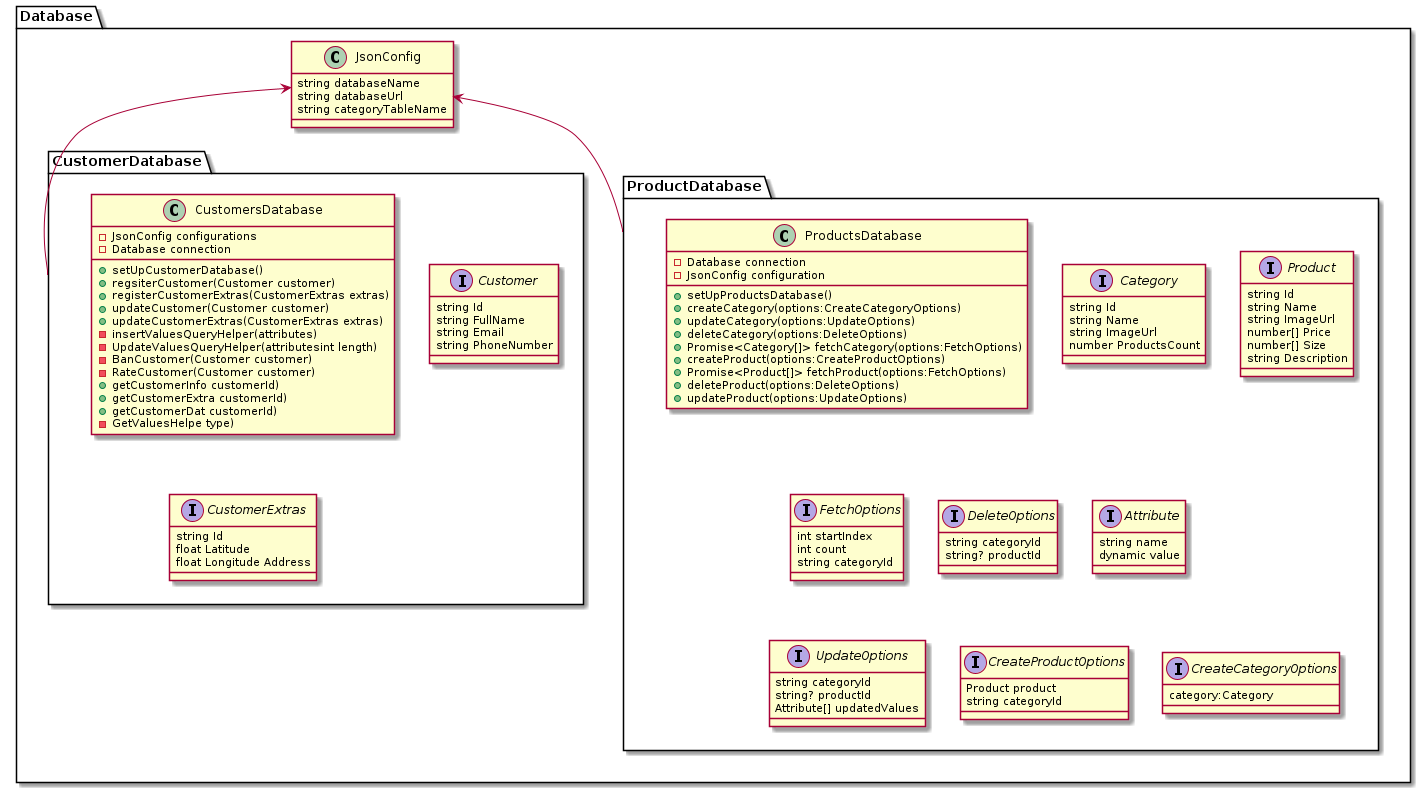
\includegraphics[scale=0.3]{./out/NodeApp/Database/Database.png}


\section{Installation}
\subsection{Dependencies}
Install \textbf{Flutter} from the official webstie \href{https://docs.flutter.dev/get-started/install}{here}\\
Install \textbf{Node package manager} from the official website \href{https://docs.npmjs.com/downloading-and-installing-node-js-and-npm}{here}\\
\subsection{Mobile App}
Clone the project from github :
\begin{verbatim}
git clone https://github.com/IDIRYACINE/online_order_client
\end{verbatim}
Navigate to the project directory and run flutter : \textbf{flutter run} 
\subsection{Node App}
Clone The project from github :
\begin{verbatim}
git clone https://github.com/IDIRYACINE/online_order_server_nodeJs
\end{verbatim}
Navigate to the project directory and run : npm start 
\subsection{React App}
Install React by running : npm install react \\
Clone The project from github : 
\begin{verbatim}
git clone https://github.com/IDIRYACINE/online_order_server_app
\end{verbatim}
Navigate to the project directory and run : npm start 



\newpage
\part{Appendix}
\textbf{Test Driven Developement}\\
Beck Kent - Test-Driven Development\\
\textbf{Code Quality}\\
Robert C. Martin - Clean Code\\
Martin Fowler - Refactoring: Improving the Design of Existing Code\\
\textbf{Domain Driven Developement}\\
Eric Evans - Domain-Driven Design: Tackling Complexity in the Heart of Software\\
\textbf{Project Architecture}\\
Mark Richards - Software Architecture Patterns\\
\textbf{Design Patterns}\\
Gang of Four Design Patterns\\
Alexander Shvets - Dive Into Design Patterns\\
\textbf{Analysis Model}\\
Martin Fowler - Analysis Patterns Reusable Object Models\\
\textbf{GitHub}\\
Scott Chacon - Pro Git\\
\end{document}

